\documentclass[a4paper,12pt]{article}
\usepackage{graphicx}
\graphicspath{{images/}}
\usepackage[x11names]{xcolor}

%\pagecolor{Cornsilk3}
%inline
{\Huge \title{Basic Biomedical Assignment-I  \\ Medical Devices}}
\author{Raj Motwani \\ Roll no- 21111042}


\usepackage[landscape]{geometry}
\begin{document}


\begin{figure}
\centering

\includegraphics[scale=0.6]{nitlogo.png}
\end{figure}
\maketitle

\clearpage


\large
\section{BILIRUBINOMETER:} 
\begin{figure}[h]

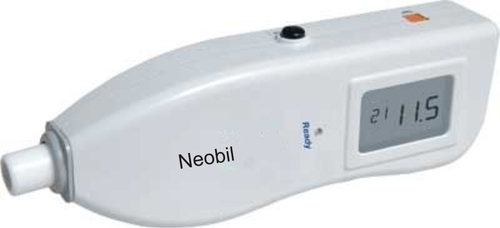
\includegraphics[scale=1.5]{bil.jpg}
\end{figure}  
 
 In healthy full-term neonates, bilirubin can rise to peak levels of
5 to 13 mg/dL between the second and fi fth days of life before
decreasing to normal levels between the fi fth and seventh days.
This produces jaundice, a yellowish discoloration of the skin, eyes,
and mucous membranes. Monitoring bilirubin concentration is
also important in children and in adults where elevated levels
may indicate a pre-hepatic, hepatic, or post-hepatic metabolic
disorder
 These devices come in a variety of physical configurations. They may be relatively small, single-purpose hand-held instruments that are simple to operate and are designed to measure the concentration of bilirubin in the blood. They are often located in neonatal intensive care units for rapid on-site bilirubin analysis, which is essential for determining a proper treatment method. Bilirubinometers may also be configured as larger benchtop analyzers or stand-alone units.
 
 Bilirubin concentrations are determined either by whole blood or serum analysis using spectrophotometric methods or by skin-reflectance measurements. The three methods of spectrophotometric analysis are the direct spectrophotometric method, the Malloy-Evelyn method, and the Jendrassik-Grof method.
 \\
 \\
 
 Blood samples are required for spectrophotometric analysis. The analysis technique depends on both the type or types of bilirubin being measured and the age of the patient (neonate versus child or adult). Cutaneous bilirubinometers do not require a blood sample. A light-emitting sensor is placed on the infant’s skin (optimally on the forehead or sternum). The reflected light is split into two beams by a dichroic mirror, and wavelengths of 455 nm and 575 nm are measured by optical detectors.
 \\
  
 Rapid changes in hydration (body water content) during therapy can cause fluctuations in blood bilirubin concentrations, making assay results uncertain. Photo-oxidation (light-induced breakdown) of bilirubin occurs if samples are exposed to light for more than a few hours. Therefore, blood samples should be protected from exposure to light.
Use and maintenance ,
User(s): Operator, medical staff
Maintenance: Medical staff; technician;
biomedical or clinical engineer
Training: Initial training by manufacturer and
manuals.
\\
 
Product specifications ,
Approx. dimensions (mm): 110 x 150 x 200
Approx. weight (kg): 3.4
Consumables: NA
Price range (USD): 3,100 - 7,000
Typical product life time (years): 6 to 8
Shelf life (consumables): NA
\\
\\
\\
 
\section{SPIROMETER:}

\begin{figure}[h]
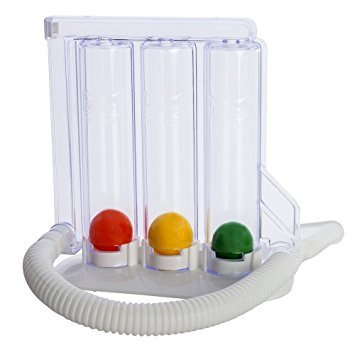
\includegraphics[scale=0.4]{spi.jpg}
\end{figure}

Spirometry (spy-ROM-uh-tree) is a common office test used to assess how well your lungs work by measuring how much air you inhale, how much you exhale and how quickly you exhale.

Spirometry is used to diagnose asthma, chronic obstructive pulmonary disease (COPD) and other conditions that affect breathing. Spirometry may also be used periodically to monitor your lung condition and check whether a treatment for a chronic lung condition is helping you breathe better.
A spirometer is an apparatus for measuring the volume of air inspired and expired by the lungs. A spirometer measures ventilation, the movement of air into and out of the lungs. The spirogram will identify two different types of abnormal ventilation patterns, obstructive and restrictive. There are various types of spirometers that use a number of different methods for measurement (pressure transducers, ultrasonic, water gauge).

It’s made of plastic and is about the size of a small notebook. It has a mouthpiece that looks like a vacuum tube. When you inhale with it, the suction will move a disc or a piston up inside a clear cylinder. The deeper you breathe, the higher the piston rises.

Most spirometers have numbers on the cylinder to show how much air you take in. They also may have a gauge to tell if you’re inhaling at the right pace.
  
  A spirometer is the main piece of equipment used for basic Pulmonary Function Tests (PFTs). Lung diseases such as asthma, bronchitis, and emphysema may be ruled out from the tests. In addition, a spirometer often is used for finding the cause of shortness of breath, assessing the effect of contaminants on lung function, the effect of medication, and evaluating progress for disease treatment.
  Breathing slowly with a spirometer allows your lungs to inflate fully. These breaths help break up fluid in the lungs that can lead to pneumonia if it’s not cleared. 
  An incentive spirometer is often given to people who’ve recently had surgery, people with lung disease, or people with conditions that fill their lungs with fluid. 
  
  After surgery. An incentive spirometer can keep the lungs active during bed rest. Keeping the lungs active with a spirometer is thought to lower the risk of developing complications like atelectasis, pneumonia, bronchospasms, and respiratory failure. 
  Pneumonia. Incentive spirometry is commonly used to break up mucus buildup that builds up in the lungs in people with pneumonia. 
  Chronic obstuctive pulmonary disease (COPD). COPD is a group of respiratory disorders that are most commonly caused by smoking. There’s no current cure, but quitting smoking, using a spirometer, and following an exercise plan can help manage symptoms. 
  Cystic fibrosis. People with cystic fibrosis might benefit from using an incentive spirometer to clear fluid buildup. A 2015 study found that spirometry has the potential to reduce pressure in the chest cavity and lower the chance of central airway collapse. 
  Other conditions. A doctor may also recommend an incentive spirometer for people with sickle cell anemia, asthma, or atelectasis.
 
 When you empty out and refill the air in your lungs, you get rid of fluid and germs that can lead to an infection. You also exercise your lungs, so that they’re able to put more oxygen into your body. That helps you to heal and avoid lung infections.

If you’re having surgery, your doctor may want you to start using your spirometer at home before you head to the hospital. If you strengthen your lungs, you’re less likely to pick up an infection there.

Experts debate the advantages of incentive spirometry. Studies show that deep breathing exercises appear to work just as well. Your doctor will suggest what may work best for you. 
  
  
  
 \section{Tissue Homogenizer:}
 
 \begin{figure}[h]
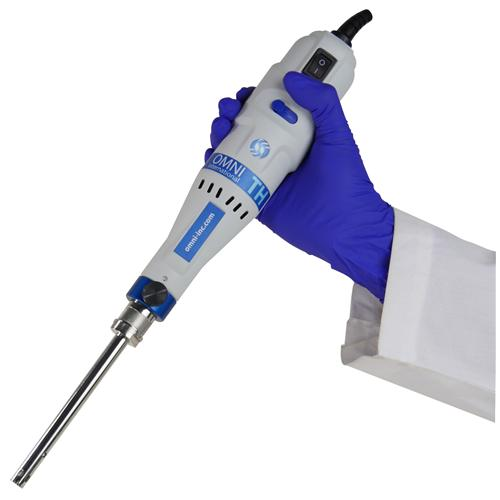
\includegraphics[scale=1]{tis.jpg}
\end{figure}
 \medspace
  
Tissue homogenization is performed regularly in labs across the world for cell and tissue preparation. This process involves lysing the cells to release intracellular contents of interest, such as proteins and nuclear components.
  
  Homogenization to break tissues down into their constituent pieces is a common first step in the lab. Depending on the desired constituent parts, different techniques may be used. For more thorough homogenization, blending of the tissue is often done first and a disruptor is then used to break the tissue down even further. Homogenizers can have dedicated functions, such as a tissue-specific homogenizer, or more general functions. If only one type of homogenization is going to be done in the lab, a tissue homogenizer may be the most economical option, otherwise investing in a homogenizer with multiple applications may be something to consider.
  \\
  There are often many different names for the same piece of mechanical homogenizing equipment, including Cell Lysor, Disperser, High Shear Mixer, Homogenizer, Polytron, Rotor Stator Homogenizer, Sonicator or Tissue Tearor.
  \\
  
  Cell fractionation is done by homogenizer to release the organelles from cell. Whereas older technologies just focused on the disruption of the material, newer technologies also address quality or environmental aspects, such as cross-contamination, aerosols, risk of infection, or noise. Homogenization is a very common sample preparation step prior to the analysis of nucleic acids, proteins, cells, metabolism, pathogens, and many other targets.
  There are several methods of cell homogenization that are commonly used. Continue reading for a brief explanation of each type of cell homogenization:
  Mechanical Disruption-
  Involve the use of rotating blades to grind and disperse cells , most effective at homogenizing cell tissues, such as liver, can homogenize small volumes, up to 20 liters ,sample loss is minimal, sonication.
  Physical disruption used to lyse cells uses high frequency sound waves to lyse cells, bacteria, and other tissue types, time consuming and best used for small volumes (<100mL),manual grinding.
    
  Mortar and pestle is used to manually grind cells, best suited for breaking apart plant tissue cells, best used for small volumes, time consuming, liquid homogenization.
  Most widely used cell disruption technique, cells are lysed by the action of being forced through a small space, suitable for use with small volumes as well as cultured cells, liquid homogenization is the most commonly used homogenization technique. In the world of liquid homogenization, there are several types of homogenizers that are designed to complete the task: Potter-Elvehjem homogenizers, French Presses, and the Dounce Homogenizer.
  \\
  \\
  
In addition, we have extensive experience in the challenges that our customers face as they transition from concept, through to R and D, clinical trials, all important FDA approval and finally, to manufacturing.
\\
\\  

  
  
\section{Ultrasonic Flowmeter:}
\begin{figure}[h]
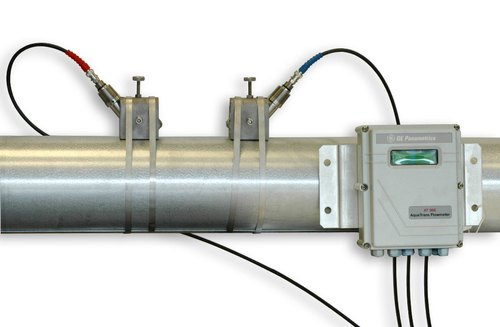
\includegraphics[scale=0.36]{ult.jpg}
\end{figure}  
  
  An ultrasonic flow meter utilizes ultrasound to measure the velocity of a fluid and is used in a variety of fluid applications. Ultrasonic flowmeters are ideal for water and other liquids. Clamp-on ultrasonic flow meters achieve high accuracy at low and high flows, save time with no pipe cutting or process shutdown, and are not affected by external noise.
  

  Ultrasonic flowmeters use sound waves to determine the velocity of a fluid flowing in a pipe. At no flow conditions, the frequencies of an ultrasonic wave transmitted into a pipe and its reflections from the fluid are the same. Under flowing conditions, the frequency of the reflected wave is different due to the Doppler effect. When the fluid moves faster, the frequency shift increases linearly. The transmitter processes signals from the transmitted wave and its reflections to determine the flow rate.
  Transit time ultrasonic flowmeters send and receive ultrasonic waves between transducers in both the upstream and downstream directions in the pipe. At no flow conditions, it takes the same time to travel upstream and downstream between the transducers. Under flowing conditions, the upstream wave will travel slower and take more time than the (faster) downstream wave. When the fluid moves faster, the difference between the upstream and downstream times increases. The transmitter processes upstream and downstream times to determine the flow rate. They represent about 12% of all flowmeters sold.
  
  This technology can be very accurate and is used for custody transfer (meaning accounting accurately for an expensive fluid) of natural gas and petroleum liquids. High turndown (can read low as a percentage of the full scale or top reading), handles high pressures, is repeatable (consistent), handles extreme temperatures, can be used clamped to the outside of a pipe without penetration, is low maintenance, highly reliable and self –diagnosing. Disadvantages can include high cost, sensitivity to stray process vibrations, problems with pipe diameter change due to buildup and clamp-on units have lower accuracy.
  Ultrasonic flowmeters do not obstruct flow so they can be applied to sanitary, corrosive and abrasive liquids. Some ultrasonic flowmeters use clamp-on transducers that can be mounted external to the pipe and do not have any wetted parts. Temporary flow measurements can be made using portable ultrasonic flowmeters with clamp-on transducers. Clamp-on transducers are especially useful when piping cannot be disturbed, such as in power and nuclear industry applications. In addition, clamp-on transducers can be used to measure flow without regard to materials of construction, corrosion, and abrasion issues. However attractive, the use of clamp-on transducers introduces additional ultrasonic interfaces that can affect the reliability and performance of these flowmeters. In particular, if not properly applied and maintained, attenuation of the ultrasonic signal can occur at the interfaces between the clamp-on transducers and the outside pipe walls, and between the inside pipe walls and the fluid.
  Ultrasonic flowmeters are available in sizes to 72 inches and larger.
  
  Ultrasonic flowmeters are commonly applied to measure the velocity of liquids that allow ultrasonic waves to pass, such as water, molten sulfur, cryogenic liquids, and chemicals. Transit time designs are also available to measure gas and vapor flow. Be careful because fluids that do not pass ultrasonic energy, such as many types of slurry, limit the penetration of ultrasonic waves into the fluid. In Doppler ultrasonic flowmeters, opaque fluids can limit ultrasonic wave penetration too near the pipe wall, which can degrade accuracy and/or cause the flowmeter to fail to measure. Transit time ultrasonic flowmeters can fail to operate when an opaque fluid weakens the ultrasonic wave to such an extent that the wave does not reach the receiver.
 The industries in order of higher to lower are oil and gas, water and wastewater, power, chemical, food and beverage, pharmaceutical, metals and mining, and pulp and paper.
 
 
\section{Pacemaker:}

\begin{figure}[h]
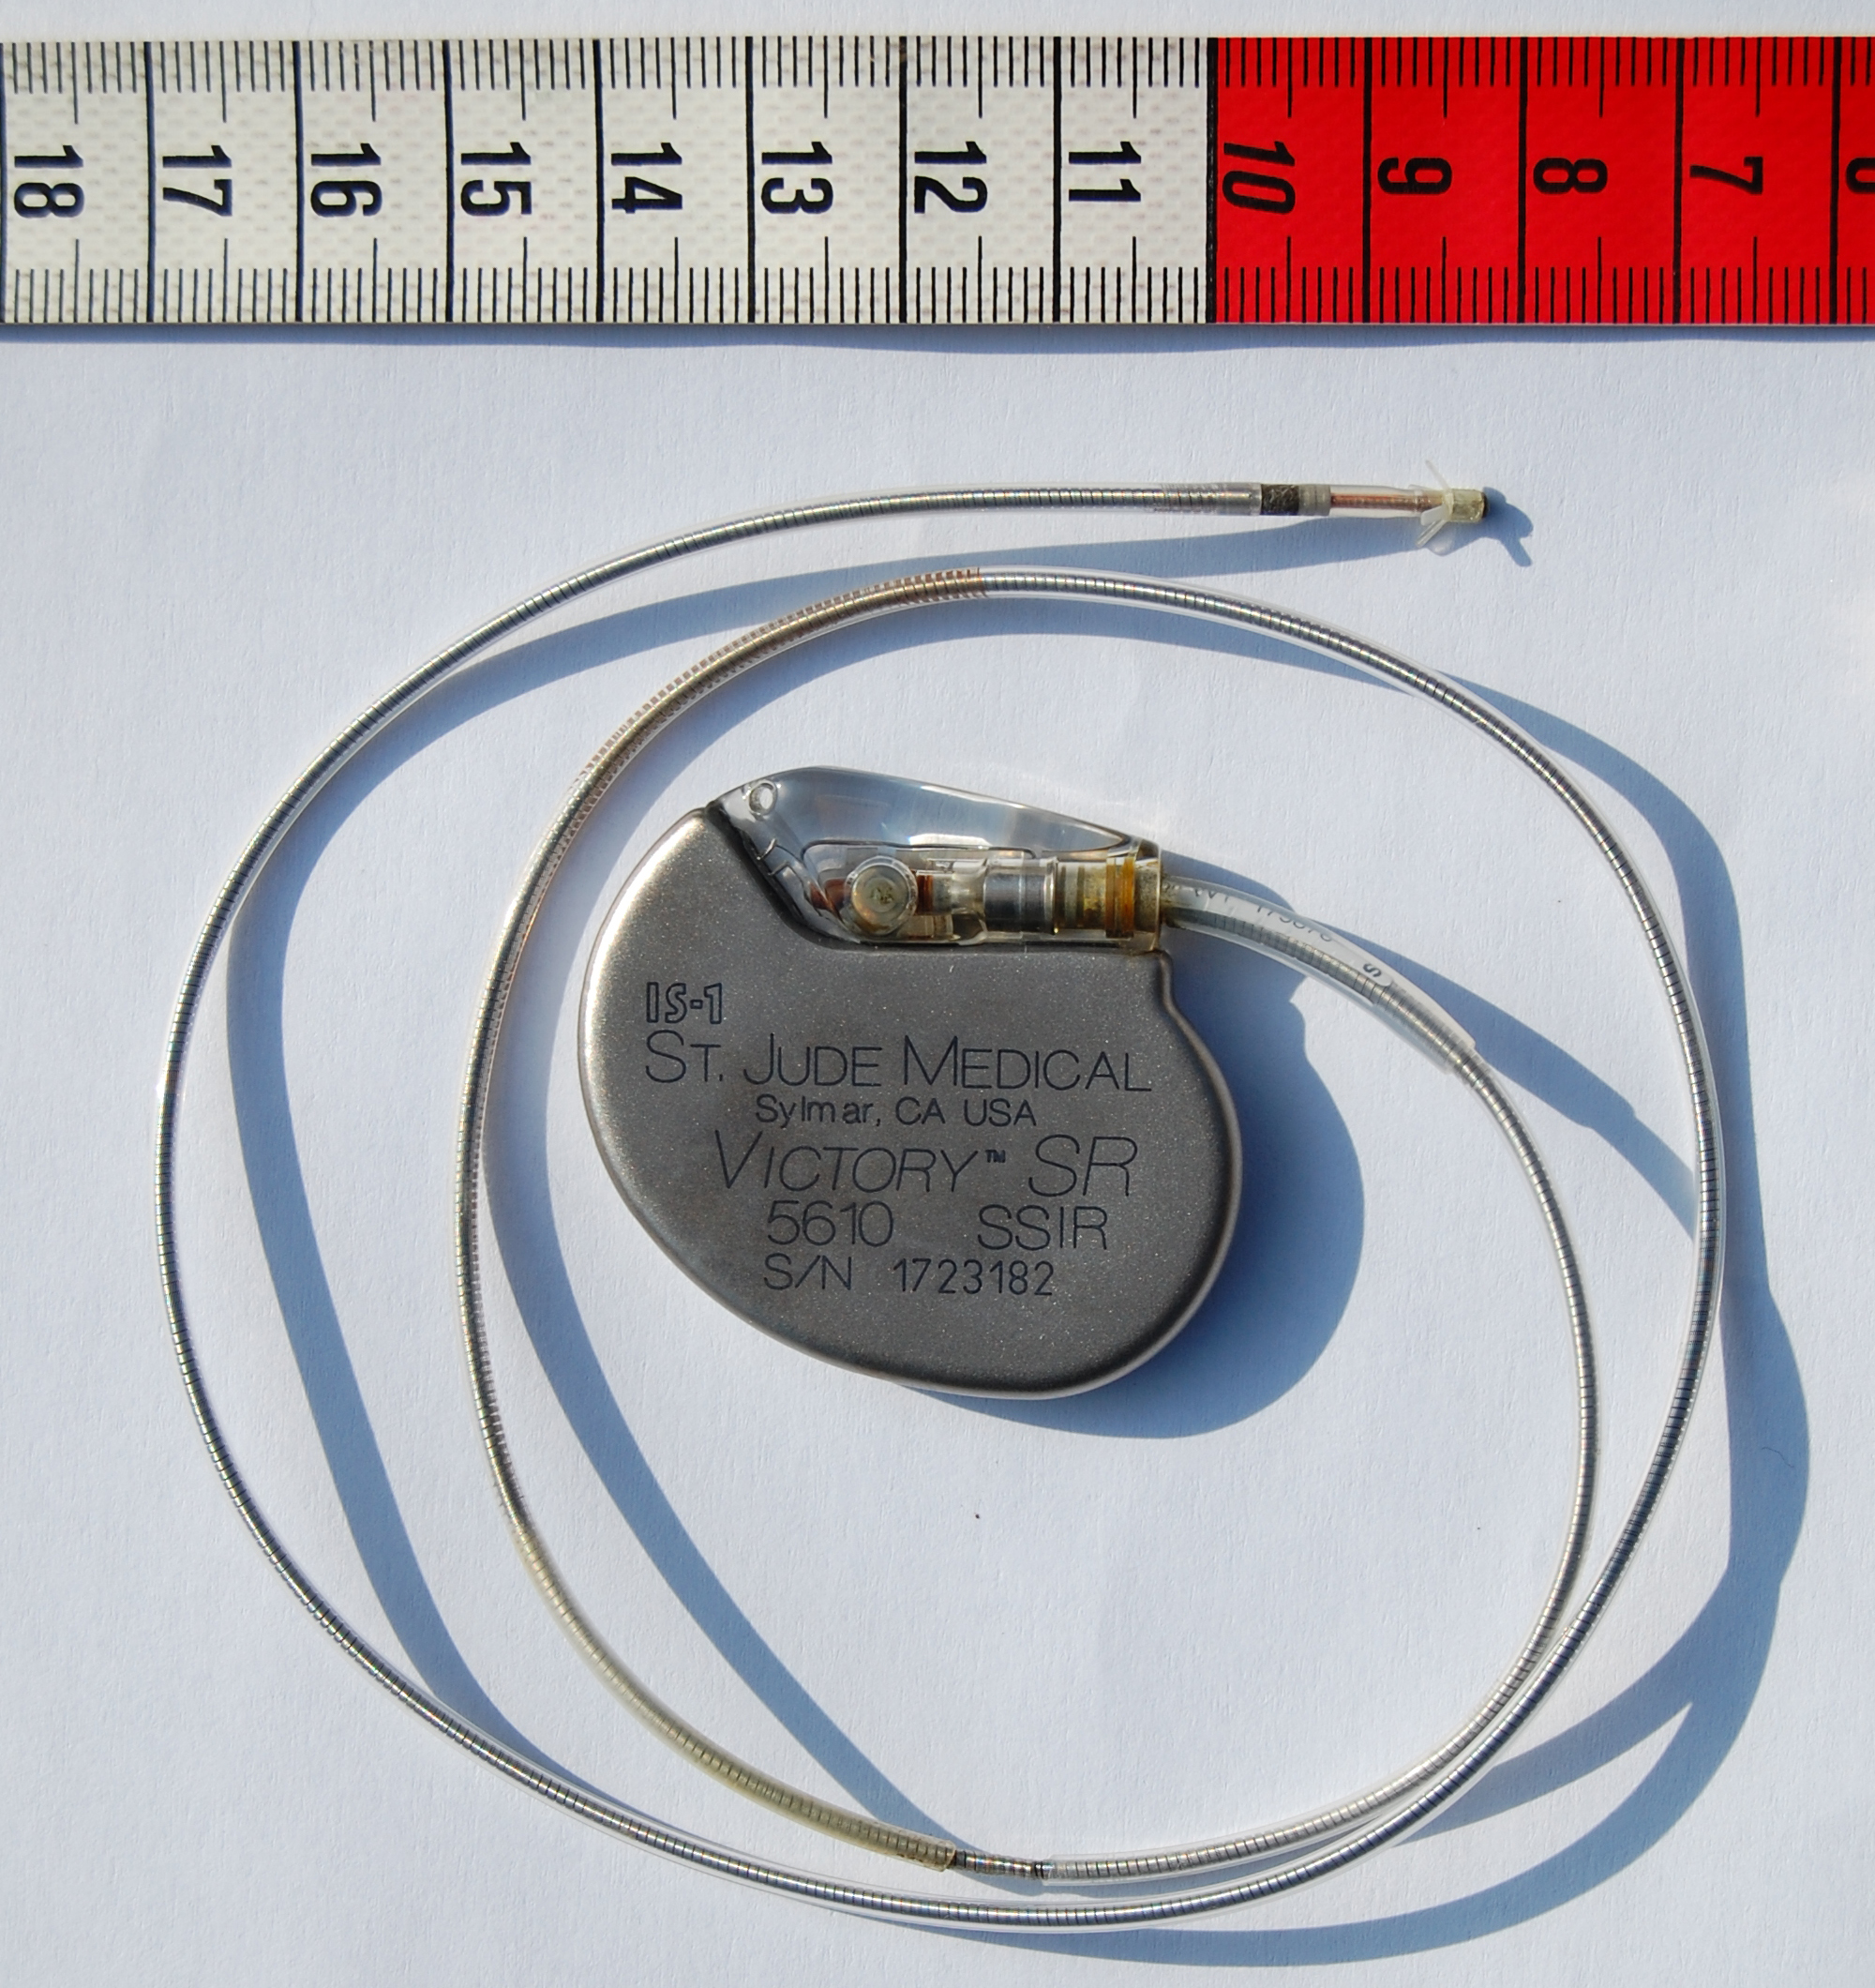
\includegraphics[scale=0.4]{pac.jpg}
\end{figure}
\medspace
 
 A pacemaker is a small device used to treat some arrhythmias. During an arrhythmia, the heart can beat too fast, too slow, or with an irregular rhythm. Pacemakers send electrical pulses to help your heart beat at a normal rate and rhythm. Pacemakers can also be used to help your heart chambers beat in sync so your heart can pump blood more efficiently to your body. This may be needed if you have heart failure.
 
 You may need a temporary (short-term) or permanent (long-term) pacemaker. A temporary pacemaker is normally inserted through a vein in the neck and remains outside your body. A permanent pacemaker is placed in your chest or abdomen. This topic focuses on permanent pacemakers.
  To get a pacemaker, you may need to stay in the hospital for a few hours or overnight. Once you are back home, your doctor may check your pacemaker remotely and schedule regular visits with you to check its activity.
 
 Many people with pacemakers can return to their regular activities within a few days. You may need to avoid certain electrical devices or devices that have strong magnetic fields.
 Pacemakers use low-energy electrical pulses to control the rate and rhythm of your heartbeat. Traditional pacemakers send the electrical pulses through wires, also known as leads. Wireless pacemakers are a newer kind of pacemaker without wires.
 Pacemakers are used to treat certain types of arrhythmias, as well as heart failure, a condition that occurs when the heart cannot pump enough blood to the body. Not everyone with an arrhythmia needs a pacemaker.
 The procedure may be planned ahead of time, or it may be done during an emergency (temporary pacemaker). You will be given medicine to make parts of your body numb or make you sleep during the procedure. 
 
 You may receive antibiotics to prevent infection and blood thinning medicine to prevent blood clots during the procedure. Different types of pacemakers require different procedures to place them.
 
 Having a pacemaker should improve symptoms caused by a slow heartbeat such as fatigue, lightheadedness and fainting. Because most of today's pacemakers automatically adjust the heart rate to match the level of physical activity, they may can allow you to resume a more active lifestyle.
 \\

Your doctor should check your pacemaker every 3 to 6 months. Tell your doctor if you gain weight, if your legs or ankles get puffy, or if you faint or get dizzy.
\\

Most pacemakers can be checked by your doctor remotely, which means you don't have to go into the doctor's office. Your pacemaker sends information to your doctor, including your heart rate and rhythm, how your pacemaker is working, and how much battery life is left.
Your pacemaker's battery should last 5 to 15 years. When the battery stops working, you'll need surgery to replace it. The procedure to change your pacemaker's battery is often quicker and requires less recovery time than the procedure to implant your pacemaker.
 
\end{document}